\begin{figure}[ht]
    \centering
    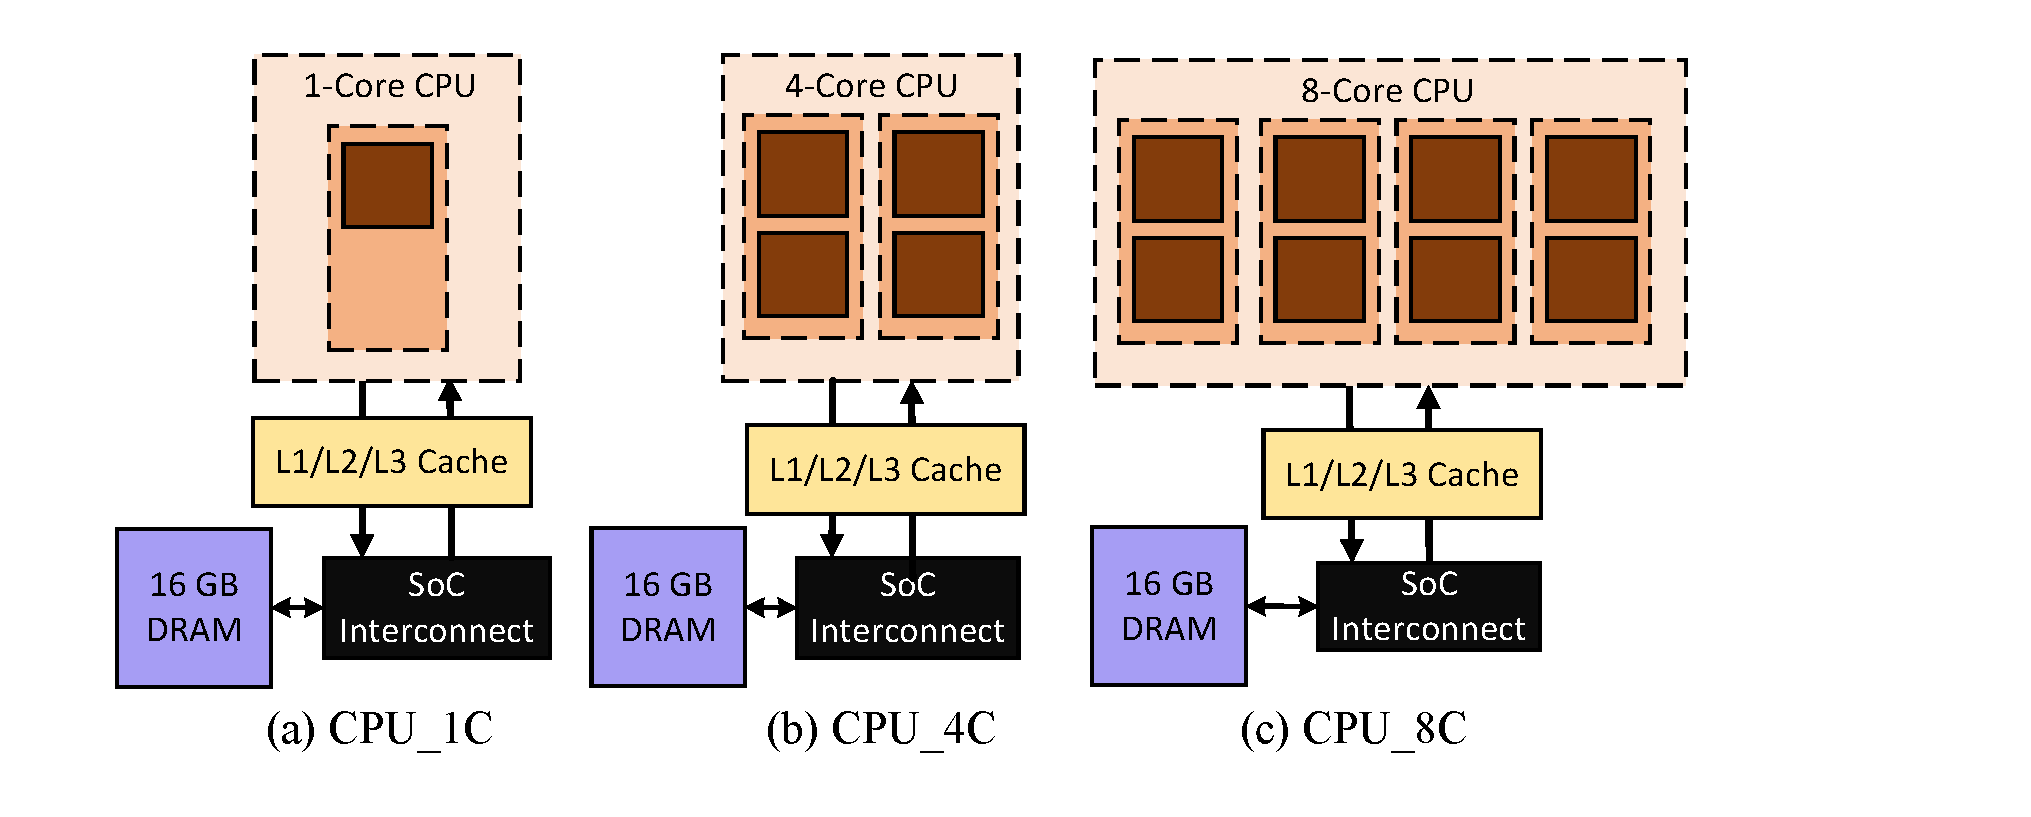
\includegraphics[width= 0.98\textwidth]{figs/mappings.pdf}
    \caption{{Different platform configurations considered in addition to Fig. \ref{fig:platform} (a).}}
    \label{fig:map_2}
    % \vspace{-5 pt}
\end{figure}

In Sections~\ref{cross_layer_approx} and \ref{lqg_control}, we mapped all the approximate tasks to a default (CPU\_8C+GPU) platform configuration (see Fig.~\ref{fig:platform}~(a)). Mapping tasks to a \gls{gpu} has runtime benefits, but it is extremely power hungry. 
The number of \glspl{cpu} online in the NVIDIA AGX Xavier platform is controlled using software-controlled power gating. We use this to introduce three new platform configurations (CPU\_1C, CPU\_4C, CPU\_8C) in Fig.~\ref{fig:map_2}. 
We report our mapping results considering design points obtained by combined application of Optim 1, 2, and 3.
\begin{figure}[h!]
    \centering
		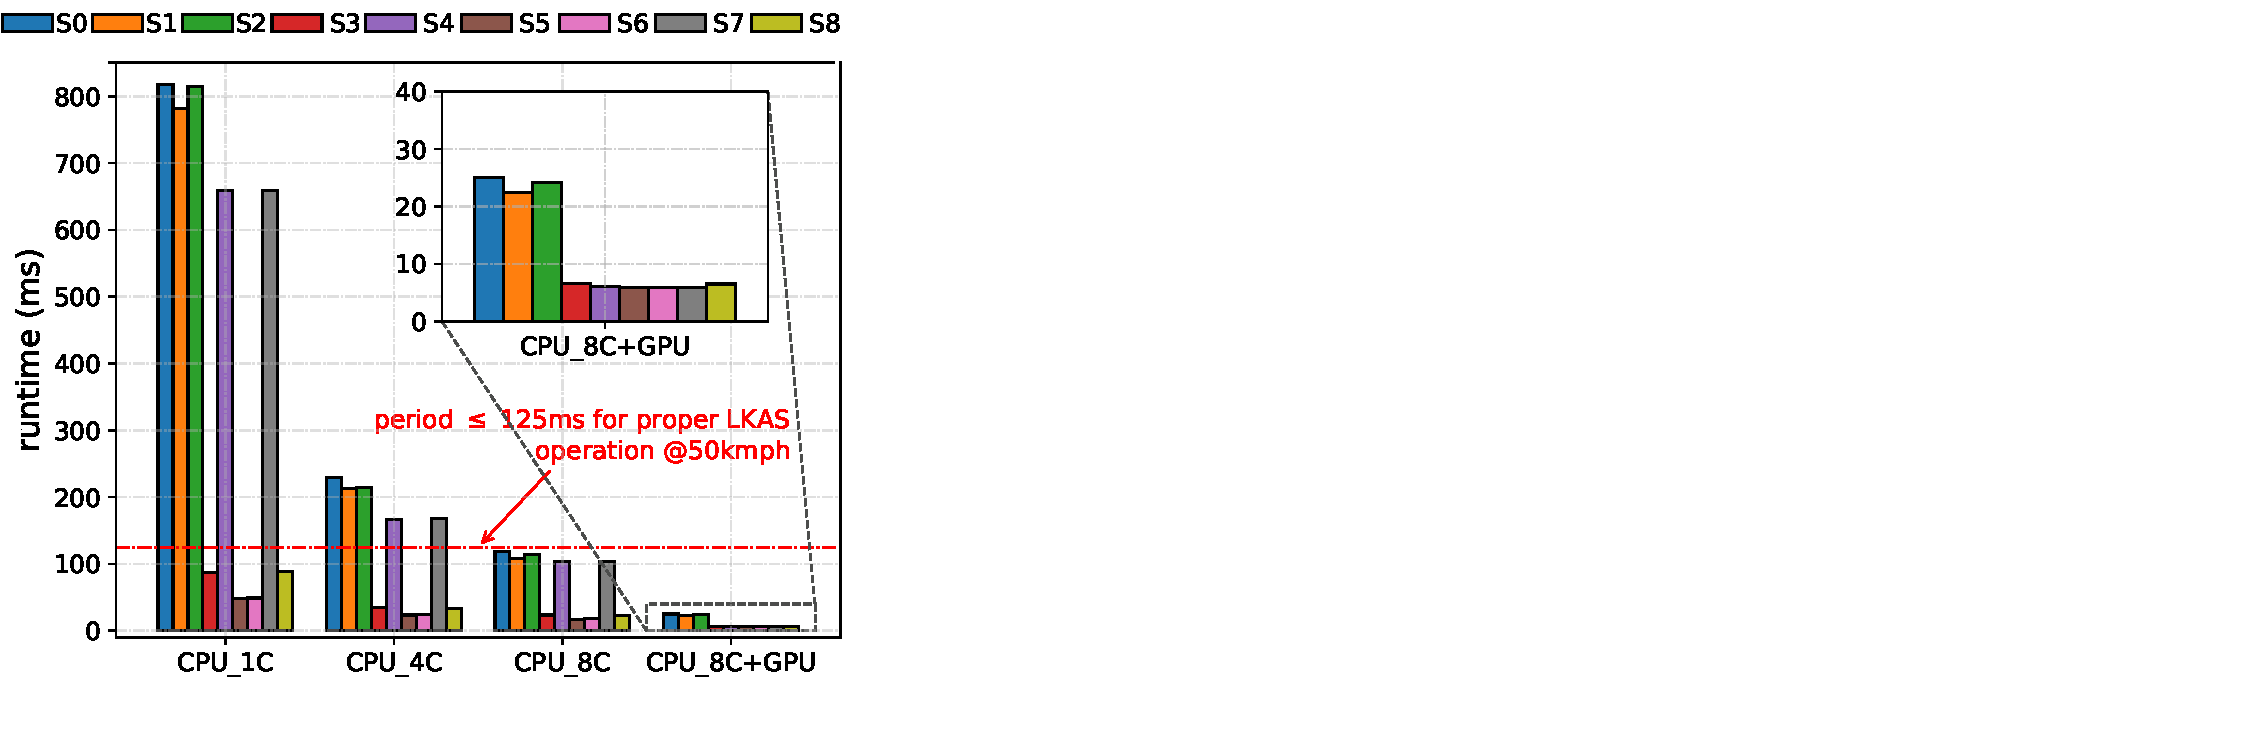
\includegraphics[width=0.8\textwidth]{figs/qoc_map_runtime.pdf}
		\captionsetup{width=0.95\linewidth}
		\caption{{Comparative analysis of the runtime implications of the different platform mappings for all approximation settings S0-S8.}}
		\label{fig:map_1}
\end{figure}
\par Fig.~\ref{fig:map_1} shows a snapshot for the timing implications of different task mappings for all approximate settings S0-S8. Sensing-to-actuation delays $\tau$ are shown on the y-axis. We have observed in our experiments that for proper \gls{lkas} operation at a vehicle speed of 50 kmph, a controller sampling period $\leq$ 125 ms is required. So, mapping the accurate setting S0 to CPU\_1C or CPU\_4C results in a vehicle crash. However, mapping approximate settings S3, S5, S6 and S8 to CPU\_1C and CPU\_4C results in desired \gls{lkas} behaviour (in \gls{qoc}-optimal mode). 
As mentioned earlier, a minimum frame rate of 8 fps (period $\leq$ 125 ms) is required for proper \gls{lkas} operation. In approximation-only mode, for each mapping, settings S1-S8 operate at the same frame rate as S0 of the corresponding mapping. Thus, all the settings result in \gls{lkas} failure for CPU\_1C and CPU\_4C. 
In \gls{qoc}-Optimal mode, settings S3, S5, S6, S8 mapped to CPU\_1C and CPU\_4C result in desired behaviour due to improved sampling period. 
These results show that approximation enlarges the design space substantially, allowing the developer to find an appropriate balance between \gls{qoc}, resource usage, and energy cost.